\documentclass[prl,showpacs, twocolumn]{revtex4-1}
\usepackage{graphicx,amssymb,color}
\usepackage[dvipsnames]{xcolor}
%\usepackage[utf8]{inputenc}
\usepackage[spanish]{babel}


\begin{document}
\title{FI3104 M\'etodos N\'umericos para la Ciencia e Ingenieria\\ Tarea 3}
\author{Camila Sandivari\\18934657-3}
\affiliation{Profesor: Valentino Gonzalez \\ Profesor Auxiliar: Felipe Pesce}
\date{\today}

\begin{abstract}
El presente reporte muestra la propia implementaci\'on del algoritmo del m\'etodo Runge-Kutta de orden $3$ para integrar el oscilador de van der Pool, que posee un amortiguamiento no lineal, por esto usaremos condiciones iniciales que nos muestran los ciclos l\'imites. Por otro lado se muestra el uso del algoritmo implementado en ode de la librer\'ia scipy.integrate para el m\'etodo Runge-Kutta de orden $4$ para integrar el sistema de lorenz (sistema de ecuaciones diferenciales ordinarias) y visualizar particularmente el atractor de Lorenz que se deriva de el modelo clim\'atico de Lorenz, m\'as especificamente de los rollos de convecci\'on en la atm\'osfera terrestre. Este es un fen\'omeno muy interesante y ejemplo cl\'asico de un atractor ca\'otico, es decir con gran sensibilidad a las condiciones iniciales. Por esto no podemos determinar el tiempo con gran exactitud ni a largo plazo, las peque\~nas variaciones en las condiciones iniciales del sistema clim\'atico lo convierte en un misterio si intentamos mirar m\'as all\'a de un par de d\'ias.\\Ambos sistemas fueron importantes aportes a la teor\'ia del Caos que a pesar de ser determinista rigurosamente hablando, nos abre las puertas a reconocer que el mundo que nos rodea es un sistema ca\'otico, nosotros mismos somos un sistema ca\'otico y por suerte nos es imposible conocer o repetir con exactitud una condici\'on inicial. 
\end{abstract}
\maketitle

\paragraph{Procedimiento}
\subparagraph{Parte 1}
Para resolver el oscilador de van der Pool debemos integrar la ecuaci\'on que describe su movimiento 

\begin{equation}
\frac{d^2y}{ds^2} = - y - \mu^* (y^2 - 1) \frac{dy}{ds}
\end{equation}

Para esto implementaremos el m\'etodo de Runge-Kutta para orden $3$ que consiste en utilizar la ecuaci\'on (2) para buscar los valores de $y(x_{n+1})$ seg\'un la deducci\'on de la ecuaci\'on (3)

\begin{equation}
y(x_{n+1}) - y(x_n) = \int_{x_n}^{x_{n+1}} f(s,y(s)) ds
\end{equation}

\begin{equation}
\int_{x_n}^{x_{n+1}} f(s,y(s)) ds \approx  \frac{h}{6} (k_{1} + 4k_{2} +k_{3})\end{equation}

Siguiendo con la deducci\'on de $y_{n+1}$ seg\'un el m\'etodo

\begin{eqnarray}
y_{0}= y(0)\\
k_{1}= f(x_{n},y_{n})\\
k_{2}= f(x_{n}+\frac{h}{2}, y_{n} +\frac{k_{1}}{2} )\\
k_{3}=f(x_{n}+h,y_{n}-k_{1-2k_{2}} )\\
y_{n+1}=y_{n} + \frac{1}{6} (k_{1} + 4k_{2} +k_{3})
\end{eqnarray}

En el caso particular de la ecuaci\'on (1) se debe aplicar el m\'etodo dos veces simult\'aneamente, para obtener la velocidad y a partir de la velocidad obtener la posici\'on. Para esto se implementa una funci\'on que recibe condiciones iniciales y entrega el arreglo de posiciones y velocidades. 

\begin{eqnarray}
1) \frac{dy}{ds} = 0; y = 0.1\\
 2) \frac{dy}{ds} = 0; y = 4.0
\end{eqnarray}

\subparagraph{Parte 2 }
La segunda parte consiste en la utilizaci\'on del m\'etodo de Runge-Kutta de orden 4 para resolver el sistema de ecuaciones diferenciales ordinarias que componen el sistema de Lorenz

\begin{eqnarray}
 \frac{dx}{ds} &= \sigma (y - x)\\
 \frac{dy}{ds} &= x (\rho - z) - y\\ 
 \frac{dz}{ds} &= xy - \beta z 
\end{eqnarray}

Al utilizar los par\'ametros $\sigma=10 $,$\beta= 8/3$,$\rho=28$ ,se integra con el m\'etodo RK4 implemetado en la librer\'ia scipy.integrate, se obtiene como soluci\'on el atractor de Lorenz . \'esto se hace mediante ode ('dotri5') que recibe la funci\'on a integrar, en este caso un sistema al que se le entregan los vectores que corresponden a las variables espaciales, dentro de un solo vector, y el tiempo. El integrador retorna el tiempo y un vector con las soluciones para los vectores entregados. Se pueden entregar condiciones iniciales y graficar en 3D , entendiendo los ejes como parte de la clase objeto.

\bigskip
\bigskip

\paragraph{Resultados}
\subparagraph{Parte 1}

Se obtienen los gr\'aficos para el espacio de fase en la figura 1, y la trayectoria en la figura 2, del oscilador de Van der Pool

\begin{figure}[h!]
\begin{center}
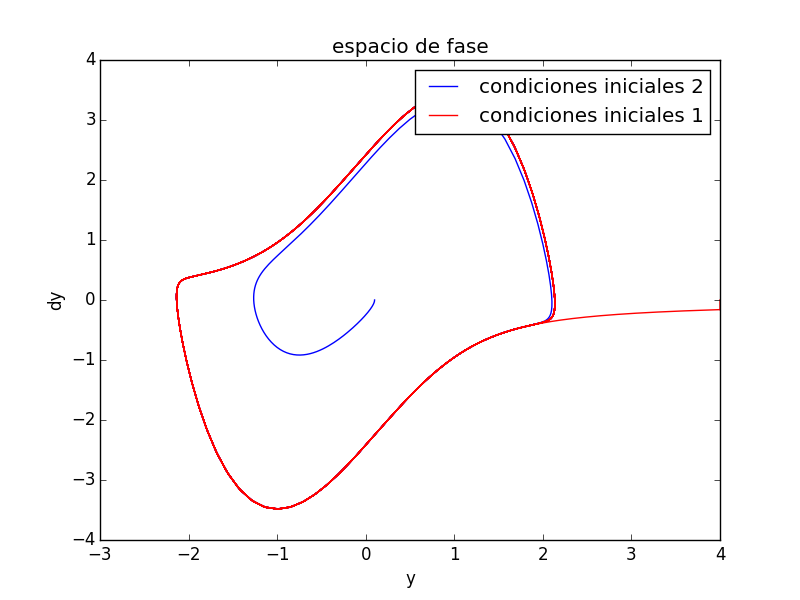
\includegraphics[width=3in]{espaciofase.png}
\caption{ Espacio de fase oscilador van der Pool}
\label{}
\end{center}
\end{figure}

\begin{figure}[h!]
\begin{center}
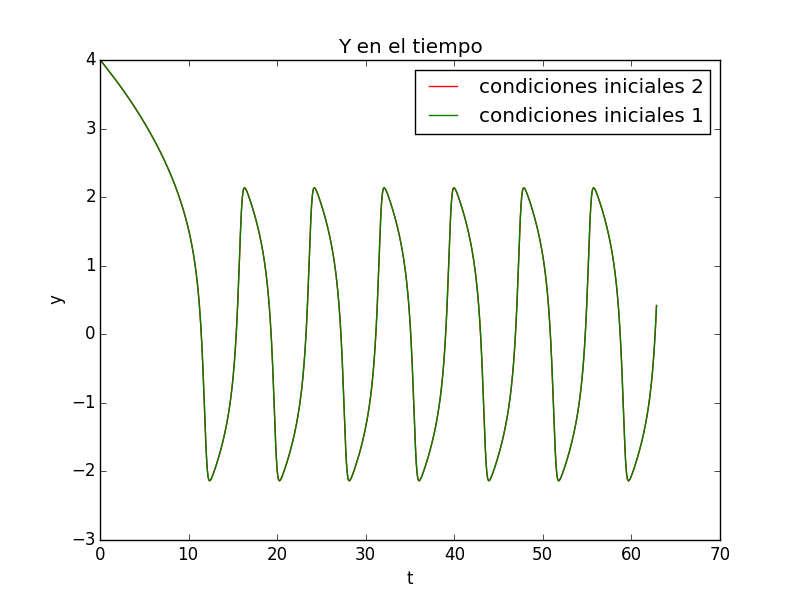
\includegraphics[width=3in]{yeneltiempo.png}
\caption{ Trayectoria versus tiempos oscilador van der Pool}
\label{ }
\end{center}
\end{figure}


\subparagraph{Parte 2 }

Se obtiene para la soluci\'on del atractor de Lorenz, un gr\'afico utilizando las condiciones iniciales $[1,1,1]$ para las posiciones $[x,y,z]$
\begin{figure}
\begin{center}
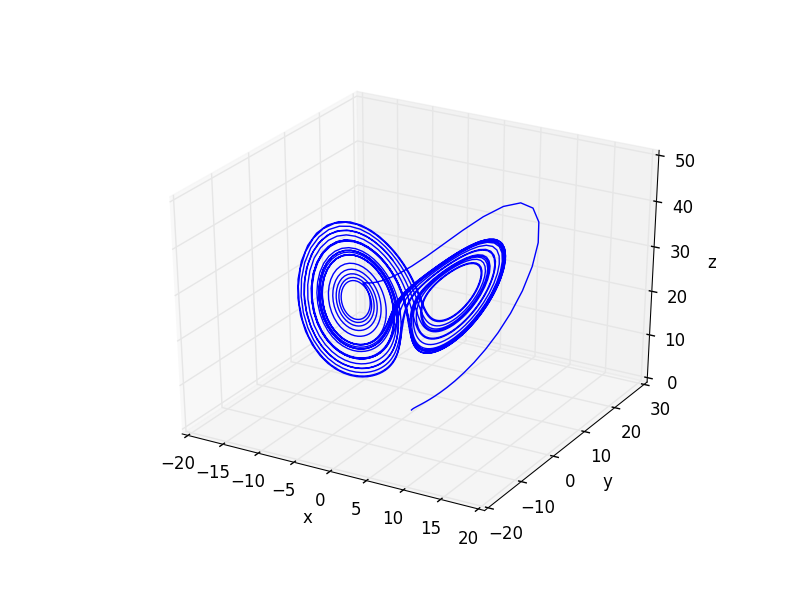
\includegraphics[width=3in]{lorenz.png}
\caption{ }
\label{ atractor de Lorenz}
\end{center}
\end{figure}

\newpage
\paragraph{Conclusiones}
El m\'etodo Runge-Kutta tanto en la versi\'on implementada como la existente en librer\'ias nos permite abordar problemas de integraci\'on bastante complejos y observar o visualizar el comportamiento de sistemas en este caso ca\'oticos que pueden ser de inter\'es.
Se obtienen resultados que coinciden con los resultados obtenidos hist\'oricamente en la resoluci\'on de estos sistemas.

\end{document}